\documentclass[12pt]{article}
\usepackage[a3paper, margin=0.6in]{geometry}
\usepackage{amsmath}
\usepackage{xcolor}
\usepackage{amssymb}
\usepackage{graphicx}     % pro obrázky
\usepackage{caption}      % pro popisky
\usepackage{float} 

\begin{document}

\section*{Domácí série II}

Vypracoval: Daniel \textit{"Randál"} Ransdorf \hfill Podpis: \rule{4cm}{0.4pt}

\begin{enumerate}
  \item \textbf{Lojza a Líza}:
    Dokažme, že každý takový mnohostěn má alespoň jednu stěnu 
    s alespoň čtyřmi sousedními (alespoň čtyřúhelníková stěna).
    Pro spor předpokládejme opak, že všechny stěny jsou trojúhelníkové,
    a pokusme se mnohostěn sestrojit.
    Začneme stěnou ABC (obr.\ 1), přidejme k ní 3 sousední trojúhelníkové stěny (obr.\ 2).
    Když takto útvar "zabalíme" (obr.\ 3) dostaneme spor, protože to bude jen čtyřstěn, nikoli mnohostěn s alespoň pěti stěnami.
    Když přidáme další trojúhelníkovou stranu, dostaneme spor,
    protože najednou u jednoho rohu budou čtyři stěny.

    Když máme toto dokázáno, můžeme konstatovat, že vždy vyhraje Líza s touto strategií:
    \begin{itemize}
      \item Líza obarví stranu, která má alespoň 4 úhly.
      \item Lojza obarví:
      \begin{itemize}
        \item Sousední stěnu:
          Líza obarví další sousední stěnu takovou, která nesousedí s Lojzovou obarvenou stěnou (obr.\ 5).
          Lízá tím získá zaručenou výhru. Protože kteroukoli stěnu Lojza obarví,
          Líza bude mít k dispozici stěnu, která sdílí roh s oběma žlutě obarvenými. Tu obarví a vyhraje (obr.\ 6).
        \item Jinou stěnu:
          Líza obarví kteroukoli ze sousedních stěn ke žluté, pak cokoli Lojza obarví,
          Líza bude mít volnou stěnu, která sdílí roh s oběma žlutě obarvenými.
          Tu obarví a vyhraje (obr.\ 7).
      \end{itemize}
    \end{itemize}

    % Obrázek 1
    \begin{figure}[H]
        \centering
        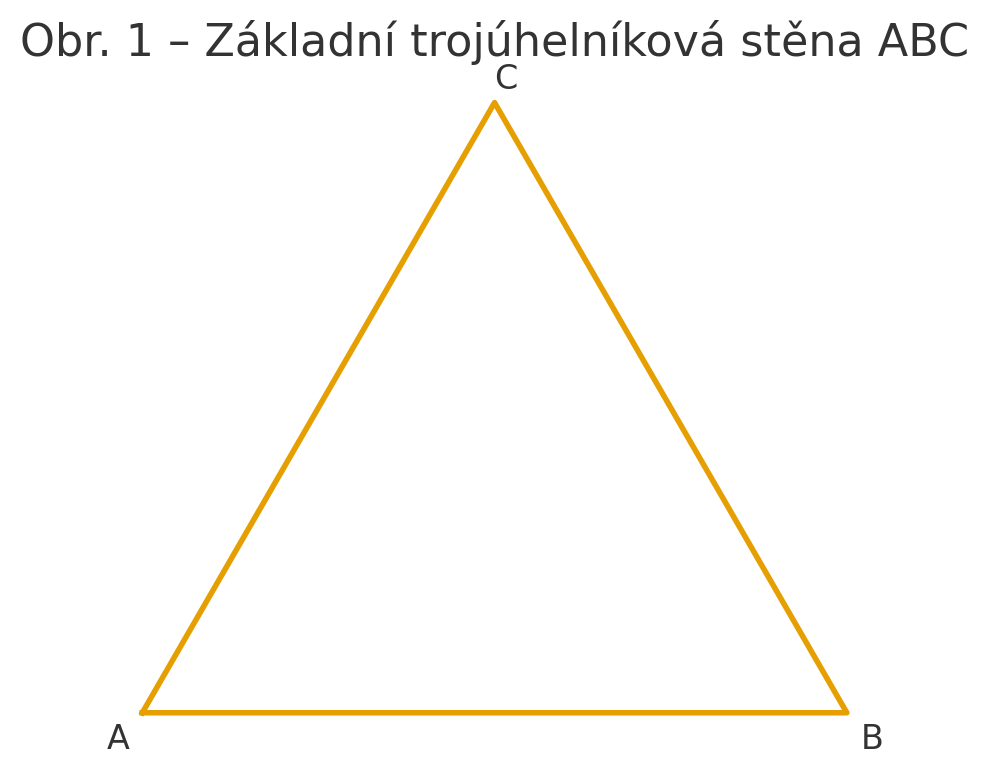
\includegraphics[width=0.2\textwidth]{domaci-2-assets/1.png}
        \caption{Obrázek 1}
        \label{fig:1}
    \end{figure}

    % Obrázek 2
    \begin{figure}[H]
        \centering
        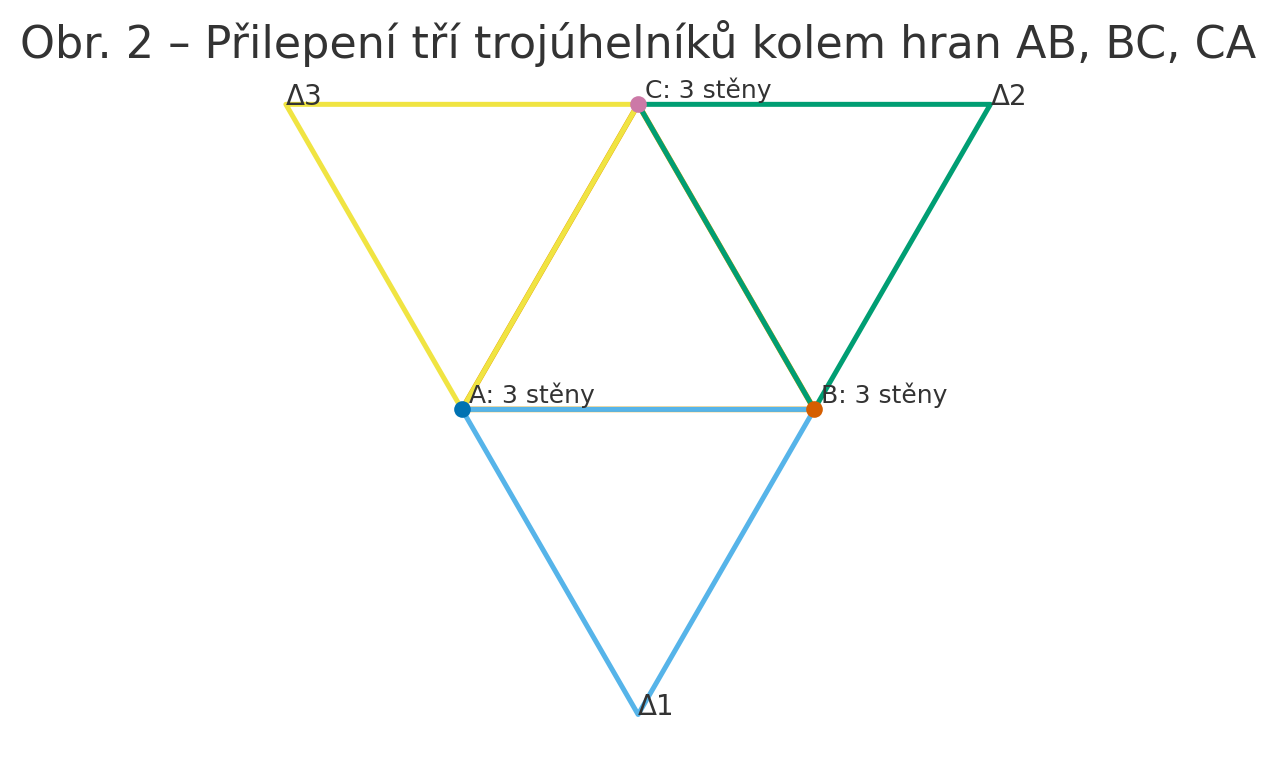
\includegraphics[width=0.2\textwidth]{domaci-2-assets/2.png}
        \caption{Obrázek 2}
        \label{fig:2}
    \end{figure}

    % Obrázek 3
    \begin{figure}[H]
        \centering
        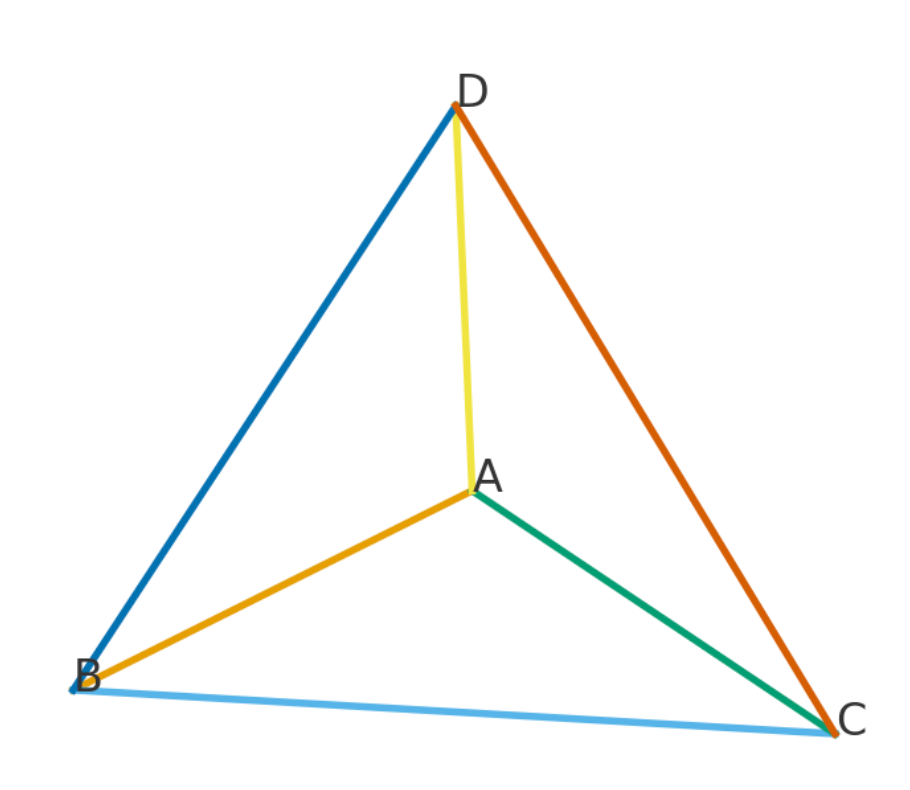
\includegraphics[width=0.2\textwidth]{domaci-2-assets/3.png}
        \caption{Obrázek 3}
        \label{fig:3}
    \end{figure}

    % Obrázek 4
    \begin{figure}[H]
        \centering
        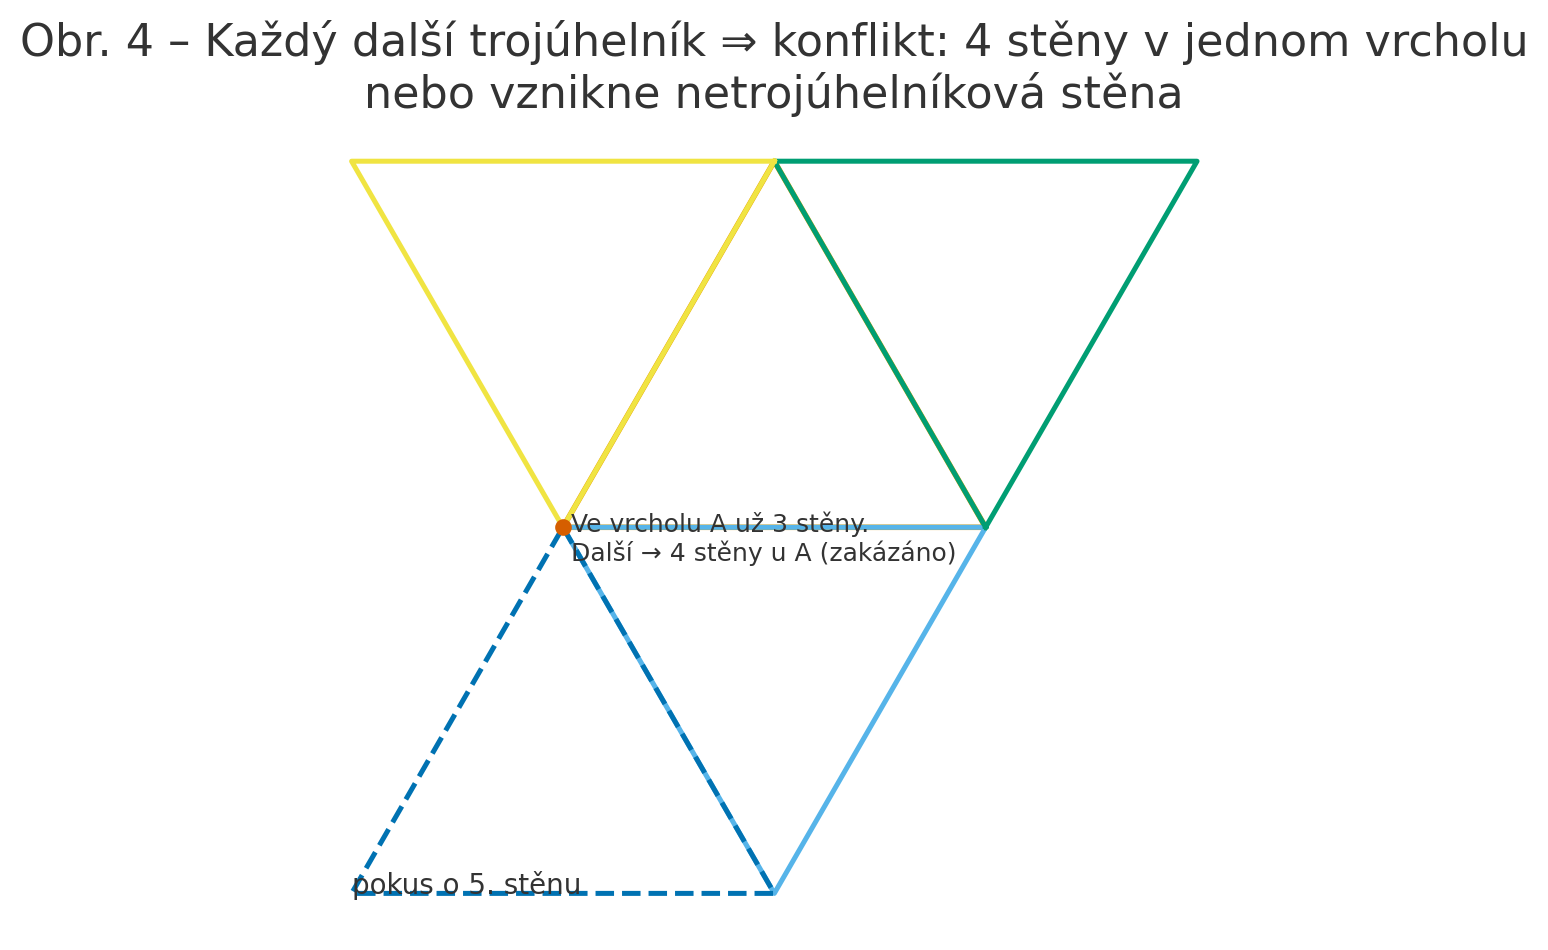
\includegraphics[width=0.2\textwidth]{domaci-2-assets/4.png}
        \caption{Obrázek 4}
        \label{fig:4}
    \end{figure}

    % Obrázek 5
    \begin{figure}[H]
        \centering
        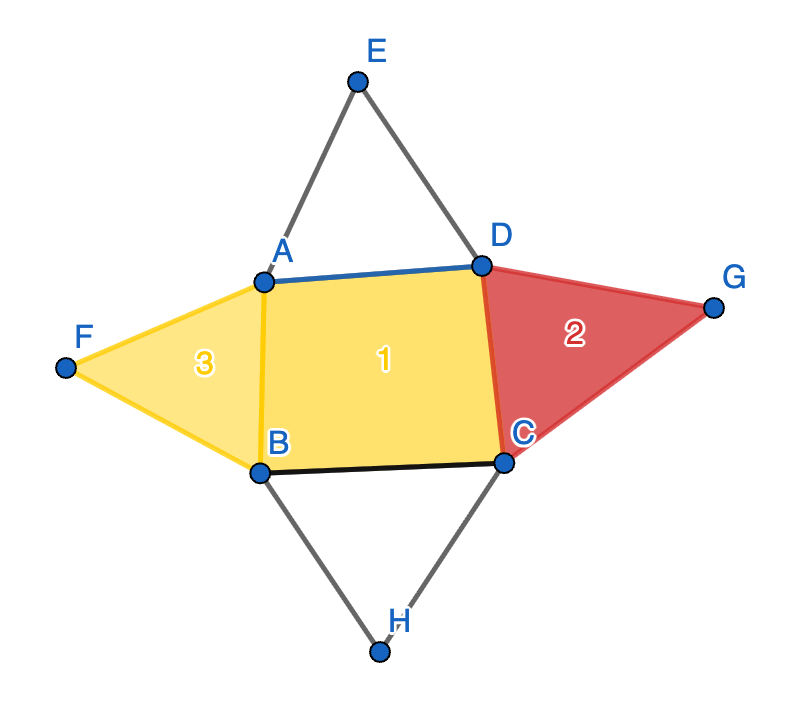
\includegraphics[width=0.2\textwidth]{domaci-2-assets/5.png}
        \caption{Obrázek 5}
        \label{fig:5}
    \end{figure}

    % Obrázek 6
    \begin{figure}[H]
        \centering
        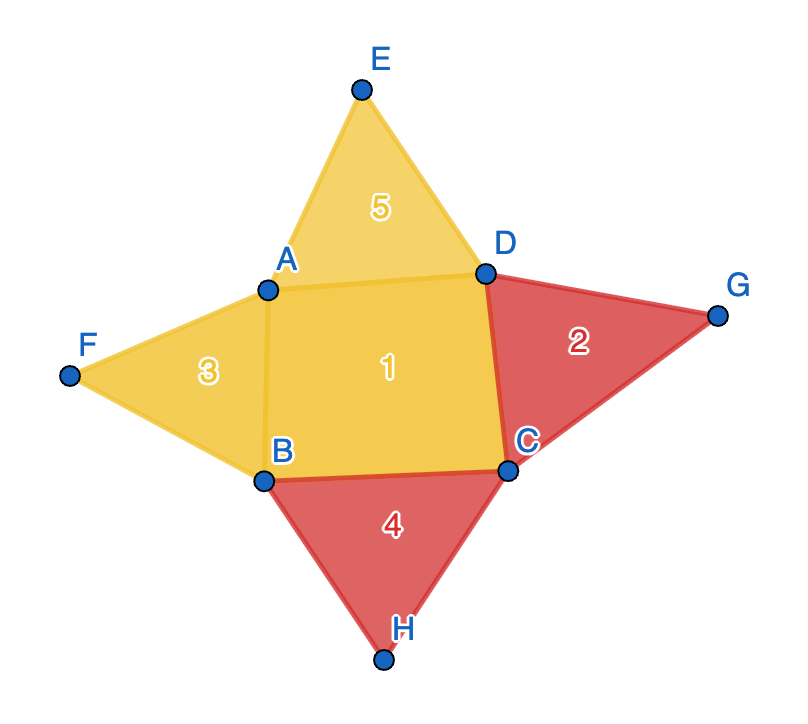
\includegraphics[width=0.2\textwidth]{domaci-2-assets/6.png}
        \caption{Obrázek 6}
        \label{fig:6}
    \end{figure}

    % Obrázek 7
    \begin{figure}[H]
        \centering
        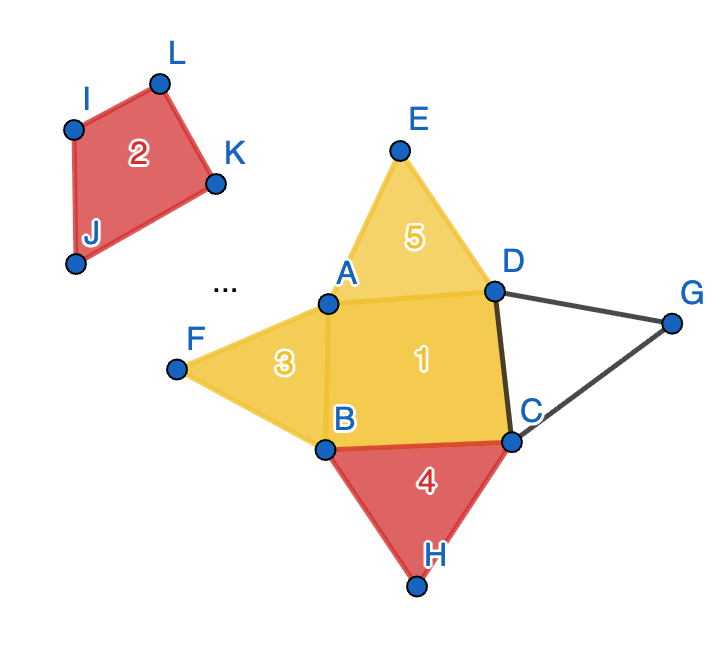
\includegraphics[width=0.2\textwidth]{domaci-2-assets/7.png}
        \caption{Obrázek 7}
        \label{fig:7}
    \end{figure}

  \setcounter{enumi}{2}

  \item \textbf{Čtverce}
    \begin{enumerate}
      \item Předpokládejme spor:
        \begin{align*}
          n(n+1)(n+2)(n+3) = x^2 \\
          (n(n+3))((n+1)(n+2)) = x^2 \\
          (n^2 + 3n)(n^2 + 3n + 2) = x^2 \\
          ((n^2 + 3n + 1) - 1)((n^2 + 3n + 1) + 1) = x^2 \\
          (n^2 + 3n + 1)^2 - 1 = x^2
        \end{align*}
        
        Plyne, že $(n^2 + 3n + 1)^2$ a $x^2$ jsou dva po sobě jdoucí čtverce. To by bylo
        možné, kdyby $x^2 = 0$ a  $(n^2 + 3n + 1)^2=1$. Ale dosazením nejmenšího $n=1$
        získáme $(1 + 4 + 1)^2 = 1$, což je zjevně spor.
        \hfill $\square$

      \item Pro 5 po sobě jdoucích čísel zapišme výraz jako:
        \[
          n(n+1)(n+2)(n+3)(n+4)
        \]
        Předpokládejme pro spor, že výraz jde odmocnit.
        Všechny přirozená čísla jsou rozložitelné na $2^{k_2}\cdot3^{k_3}\cdot z$, kde $k_2,k_3 \in \mathbb{N}_0$.
        Pokud je v některém z pěti zbytků $z$ nějaký další prvočíselný dělitel $p \ge 5$, bude zjevně v
        pěti-číselné řadě pouze jednou. Žádné další z čísel nebude dělitelné $p$. To dané číslo dělitelné $p$
        musí mít ve svém prvočíselném rozkladu sudý počet $p$, aby byl součin odmocnitelný.
        Z toho plyne předpoklad, že aby byl součin odmocnitelný, musí každé číslo splňovat, že jeho $z$ je odmocnitelné.
        Čísla můžeme rozdělit do čtyř skupin podle rozkladu na součin $2^{k_2}\cdot3^{k_3}\cdot z$:
        \begin{enumerate}
          \item \underline{Exponent $k_2$ je lichý, exponent $k_3$ je lichý}:
            Můžeme zapsat jako $2\cdot3\cdot(2^{k_2-1}\cdot3^{k_3-1}\cdot z)$, kde závorka jde odmocnit, protože 2 a 3
            jsou najednou na sudou mocninu a $z$ musí být podle předpokladu také odmocnitelné.
            Závorku tedy označme jako $a^2$, kde $a\in\mathbb{N}$, dostaneme $6\cdot a^2$
          \item \underline{Exponent $k_2$ je sudý, exponent $k_3$ je lichý}:
            Můžeme zapsat jako $3\cdot(2^{k_2-1}\cdot3^{k_3-1}\cdot z)$, kde závorka jde odmocnit, protože 2 a 3
            jsou najednou na sudou mocninu a $z$ musí být podle předpokladu také odmocnitelné.
            Závorku tedy označme jako $a^2$, kde $a\in\mathbb{N}$, dostaneme $3\cdot a^2$
          \item \underline{Exponent $k_2$ je lichý, exponent $k_3$ je sudý}: Obdobně můžeme přepsat na $2\cdot a^2$.
          \item \underline{Exponent $k_2$ je sudý, exponent $k_3$ je sudý}: Obdobně můžeme přepsat na $a^2$.
        \end{enumerate}

        Máme 5 přirozených čísel, ale jen 4 skupiny. Jedna ze skupin musí tedy být v součinu alespoň dvakrát.
        Rozdělme případy podle toho, která ze skupin, se vyskytuje v pětici dvakrát. Dokažme ve všech možnostech spor:
        \begin{enumerate}
          \item \underline{$6a^2$}: V pětici tedy máme alespoň čísla $6a_1^2, 6a_2^2$, kde $a_1,a_2\in\mathbb{N}$. Pětice je po sobě jdoucí, tedy
            musí platit $|6a_1^2 - 6a_2^2| \le 4$. Plyne $|a_1^2 - a_2^2| \le \frac{2}{3}$, což je spor, protože neexistuje dvojice
            přirozených čísel, kterých čtevrce jsou od sebe vzdálené méně než $\frac{2}{3}$.
          \item \underline{$3a^2$}: V pětici máme čísla $3a_1^2, 3a_2^2$, kde $a_1,a_2\in\mathbb{N}$.
            Obdobně získáme rovnici $|a_1^2 - a_2^2| \le \frac{4}{3}$, což je stejný spor, nejmenší vzdálenost mezi čtverci v $\mathbb{N}$
            je 3 (mezi $1^2$ a $2^2$).
          \item \underline{$2a^2$}: Obdobně získáme rovnici $|a_1^2 - a_2^2| \le 2$, což je opět stejný spor.
          \item \underline{$a^2$}: Obdobně získáme rovnici $|a_1^2 - a_2^2| \le 4$, což by fungovalo jen, pokud $a_1=1,a_2=2$,
            ale tuto možnost vyloučíme, protože posloupnost s těmito čísly
            také není odmocnitelná ($1\cdot2\cdot3\cdot4\cdot5 = 120 \ne x^2, x\in\mathbb{N}$).
        \end{enumerate}
      \hfill $\square$
    \end{enumerate}
  
  \setcounter{enumi}{4}

  \item \textbf{Součet $k$ 101-úhelníkových úhlopříček}
    
    Vyřešme extrémní příklad, kde bude nejvíce úhlopříček o délce $\approx 0$, dále ukažme,
    že u všech jiných 101-úhelníků bude potřeba úhlopříček méně, aby byla splněna nerovnost v zadání.

    \begin{figure}[H]
        \centering
        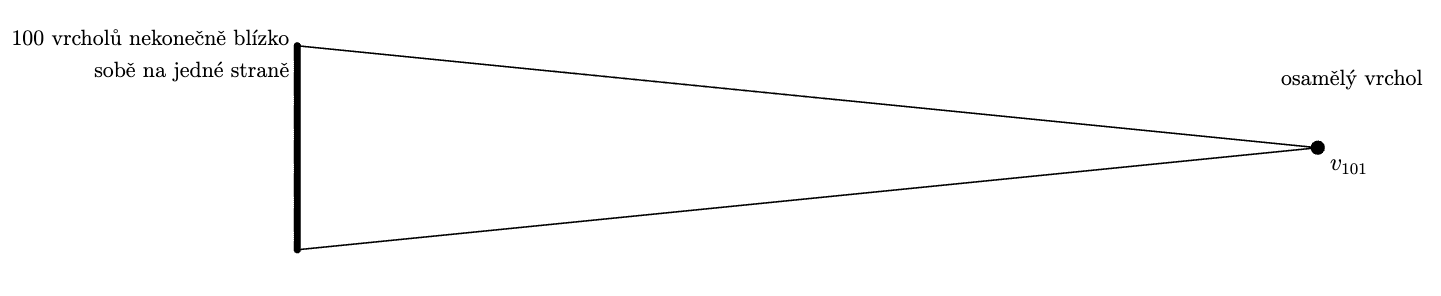
\includegraphics[width=0.8\textwidth]{domaci-2-assets/8.png}
        \caption{Obrázek 8}
        \label{fig:8}
    \end{figure}
    

    V tomto případě (obr. 8) bude 98 úhlopříček o nějaké délce $\approx d>0$ a zbytek o délce $\approx 0$.
    Celkově bude ve 101-úhelníku 4949 úhlopříček, dle vzorce:
    \[
    \frac{n(n-3)}{2}
    \]
    Máme tedy 4851 úhlopříček se součtem délek $\approx 0$, aby byl součet větší nebo roven, musíme jich vzít
    4900, abychom tam měli alespoň 49 úhlopříček o délce $\approx d$. Součet 4900 délek musí tedy být větší nebo roven $49d$,
    součet zbylých 49 délek musí být zjevně menší nebo roven $49d$.
    Jakýmkoliv znatelným roztažením těch 100 bodů vzniknou další úhlopříčky s nezanedbatelnou délkou.
    Tím se některé z krátkých úhlopříček prodlouží, takže součet délek libovolných k úhlopříček nebude klesat
    a podmínka se možná bude dát splnit už pro menší k. Proto horší konfigurace než tento shluk 100 bodů neexistuje
    a při jakémkoli znatelném roztažení se potřebné k nezvyšuje.
    Tedy nejmenší číslo $k$ je 4900.

\end{enumerate}

\end{document}
